\section{Introduction}
\label{section:introduction}

The imperative to scale Ethereum is driven by its growing user base and the 
increasing complexity of applications built on its platform. The current 
strategy to address the scaling issues leans heavily on the concept of modularity 
through rollups and data availability and consensus layers.

While this approach has shown promise, existing solutions introduce several drawbacks:
\begin{itemize}
    \item \textbf{Fragmentation}:
      Rollups are separated from each other by design. 
      This leads to fragmentation in terms of security, liquidity, and data consistency.
    \item \textbf{Updates in zkEVMs}:
        The dynamic nature of zkEVMs brings regular updates that may lead 
        to potential security vulnerabilities.
    \item \textbf{Applications Redeployments}:
        Users have to redeploy their applications from Ethereum to L2, which in
        the same time causes liquidity fragmentation which leads us to the first
        point. 
\end{itemize}

In addressing Ethereum's scalability and fragmentation challenges, 
we propose a new layer-2 (L2) concept, \textit{zkSharding}.
This solution merges Zero-Knowledge proofs with a sharding mechanism and blends 
a bunch of other \nil technologies into it. 

Key aspects include:
\begin{itemize}
    \item \textbf{"zkRollup with Sharding" for Horizontal Scalability}:
    The core of zkSharding is a blend of zkRollups and sharding, enabling extensive 
    horizontal scalability without compromising security or reducing efficiency. 
    This approach counters the limitations of vertical scaling (L3, L4, etc.),
    significantly reducing data and liquidity fragmentation.
    \item \textbf{Direct Ethereum data access}:
    The ability to call Ethereum's original data from L2 applications allows us 
    to reuse already deployed applications. Direct access to L1 data from L2 
    ensures a more unified and seamless environment.
    \item \textbf{Type-1 zkEVM Compiled via zkLLVM from in-Production EVM}:
        zkEVM's, being often implemented from scratch to replicate the actual
        state transition executor logic (EVM) pose security risks as the circuit
        is very large, very complicated and hardly auditable. zkSharding relies
        on a zkEVM circuit compiled by zkLLVM circuit compiler from a 
        production-grade EVM without manual circuit reimplementation which
        reduces security risks.
\end{itemize}

We envision zkSharding as a step forward in blockchain modularity, aligning with 
Ethereum's principles and offering a scalable, integrated solution.

\nil zkSharding solution provides the follwing properties:
\begin{enumerate}
    \item \textbf{Scalability}: 
    \begin{enumerate}
        \item No scalability limitations as the execution is parallel. 
        Throughput around ~60k transfers per second with around 400
        nodes.
        \item Competitive marketplace-based proof generation guarantees
        fastest L1-finality and chepest generation costs.
    \end{enumerate}
    \item \textbf{Unified Liquidity/Security}:
    \begin{enumerate}
        \item No security/liquidity fragmentation as each shard is
         a part of the wholistic cluster. 
        \item Reduction of a need to migrate liquidity from Ethereum as
        \texttt{=nil;} provides transparent access to its' data for
        applications.
    \end{enumerate}
    \item \textbf{Security}:
    \begin{enumerate}
        \item State transitions secured by \texttt{=nil;}'s 
            zkEVM compiled via zkLLVM.
            It provides auditable security (e.g. constraints security) as the code is 
            easily inspectable since zkEVM circuits are compiled from a 
            production-used EVM implementation in high-level language
            and not written manually.
        \item Liveness security guaranteed with native staking or restaking existing staking pools (e.g. Lido) TVL.
        \item Decentralized from day one thanks to combination of Ethereum staking and Proof Market.
            See Section \ref{section:proof-market} for details.
    \end{enumerate}
    \item \textbf{Functionality}:
    \begin{enumerate}
        \item A Type-1 zkEVM\footnote{
            \url{https://vitalik.ca/general/2022/08/04/zkevm.html}
        }, fully EVM bytecode-equivelent.
        \item An environment tailored for applications 
            that have high demands related to time, memory, 
            and algorithmic complexity. 
            Examples include Decentralized Exchanges (DEXes) 
            or Proof Market\footnote{\url{proof.market}}.
    \end{enumerate}
\end{enumerate}

% \todo[inline]{May be it would be a good idea to show how it works from the client DApp point of view. 
% May be highlight some important cases, such as redeploing existing Eth contracts, for instance.
% Also, we could talk a little bit more about features, which required by DEX or any other types of clients if we understand them. S.K.}

\subsection{Overview}

As illustrated in Figure \ref{figure:overview}, 
the state of \protocol is partitioned into the main shard and several secondary 
shards. The main shard's role is to synchronize and consolidate data from the 
secondary shards. It uses Ethereum both as its Data Availability Layer and as a 
verifier for state transition proofs, similar to typical zkRollups operations. 
For a comprehensive understanding of the sharding approach, refer to Section 
\ref{section:sharding}.

Secondary shards function as "workers", executing user transactions. 
These shards maintain unified liquidity and data through a cross-shard messaging 
protocol, eliminating any fragmentation amongst them. 

Each shard is supervised by a committee of validators. There is a periodic 
rotation of these validators across shards. In addition, updates to a shard's 
state are verified to the main shard using zkEVM (see \ref{section:zkvm} for a 
detailed explanation).

Users have direct access to Ethereum data, thanks to the Ethereum Data Provider 
linked to every shard. This data is validated using zkBridge.

\begin{figure}[h]
    \centering
	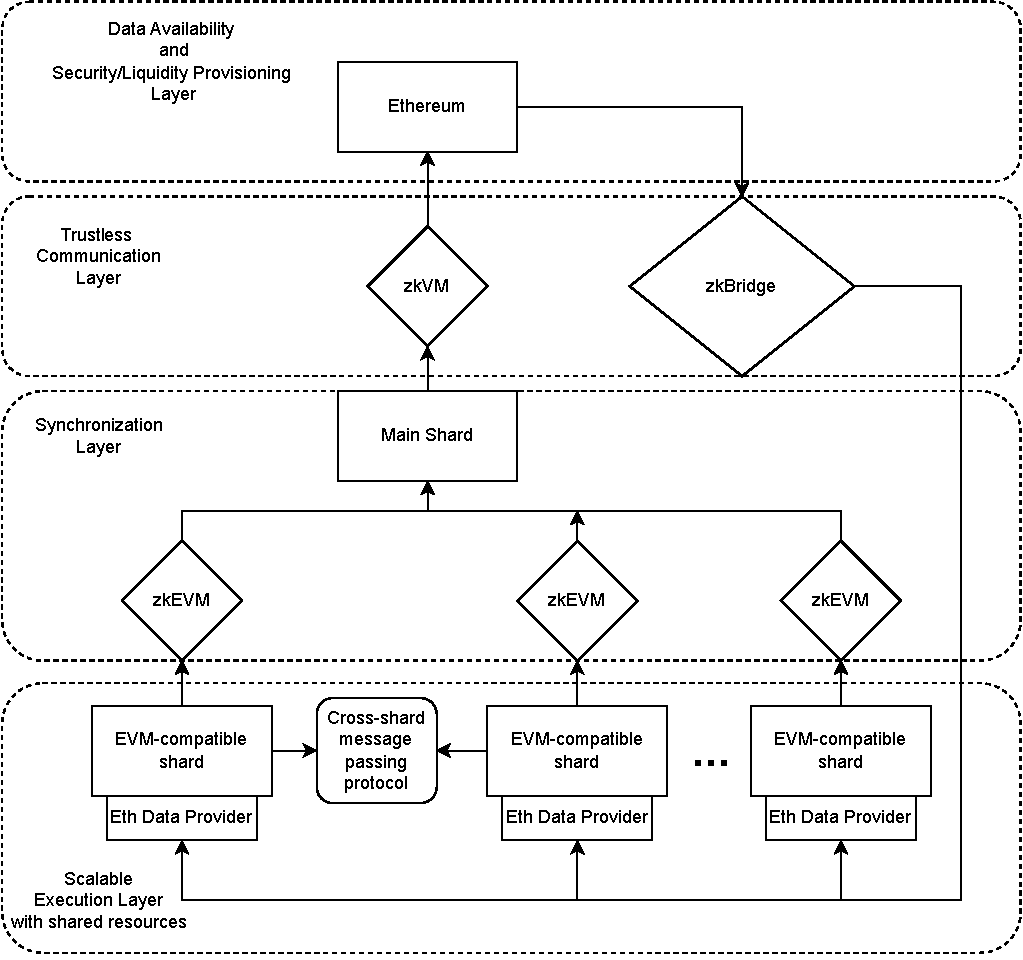
\includegraphics[scale=0.55]{figures/overview.pdf}
    \caption{\protocol overview}
     \label{figure:overview}
\end{figure}

To illustrate the transaction flow from initiation 
 by a user to confirmation on Ethereum, consider the following steps:
\begin{enumerate}
    \item The user signs a transaction $tx$ and dispatches it to the network.
    \item Validators in shard $S$, where the user's wallet is located,
        place $tx$ into the mempool.
    \item These validators then create a new block $B_{S}^{1}$.
    \item The hash of $B_{S}^{1}$ is recorded on the main shard within block $B_{M}^{1}$.
    \item A state transition proof for $B_{S}^{1}$ is 
        produced and verified by the main shard in block $B_{M}^{2}$.
    \item A state transition proof for $B_{M}^{2}$
        is sent to Ethereum for verification 
        and coupled with the necessary data for ensuring data availability.
    \item Once this process is complete, 
        $tx$ achieves confirmation by Ethereum.
\end{enumerate}

This outline assumes that the user's transaction does not
 activate the cross-shard messaging protocol.
However, in this case the transaction flow remains the same with a 
 difference that user's transaction triggers a creation of new 
 transactions on other shards. 
